\SourceLeaf{252}%
\noindent auf der Ebene nur \textls{eins}, mit \textls{zwei} Seiten; so muss es also für $a$ in der Ebene
\textls{einen} symmetrischen Punkt $a'$ und für $b$ ein $b'$ geben; und muss $ab$ mit
$a'b'$ zusammenfallen, wenn ich \textls{umklappe}, und, im allgemeinen, \textls{nur} durch
Umklappen. Symmetrisches von Symmetrischem wird hier congruent. Kommt
nun die dritte Dimension hinzu, und liegen \textls{beiderseits} $c$ und $c'$ über $a$
und $a'$, so fallen beim Umklappen auch $c$ und $c'$ auf verschiedene Seiten
der Ebene u.\,s.\,w. --- Ich meine, auf diesem Wege liesse sich eine
anschauliche Überzeugung gewinnen.

\Needspace{7\baselineskip}
\begin{center}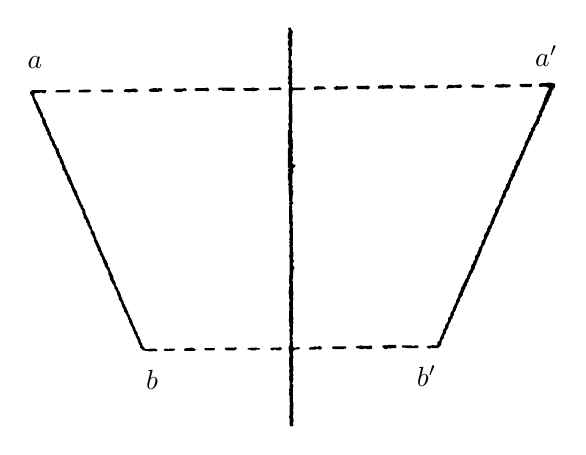
\begin{tikzpicture}[x=0.00684932cm,y=-0.00684932cm]
\fill[even odd rule] (267,608) -- (268,609) -- (284,609) -- (285,608) -- (287,608) -- (288,606) -- (287,605) -- (277,605) -- (276,606) -- (274,606) -- (273,605) -- (269,605) -- (267,607) -- cycle
(342,605) -- (342,606) -- (344,608) -- (359,608) -- (362,606) -- (361,604) -- (343,604) -- cycle
(422,605) -- (423,607) -- (427,607) -- (428,608) -- (437,608) -- (438,607) -- (444,607) -- (445,606) -- (444,604) -- (440,604) -- (439,603) -- (434,603) -- (433,604) -- (431,603) -- (428,603) -- (427,604) -- (423,604) -- cycle
(326,606) -- (319,603) -- (315,603) -- (314,604) -- (308,604) -- (307,605) -- (305,605) -- (304,607) -- (306,609) -- (324,609) -- (326,607) -- cycle
(486,604) -- (482,602) -- (480,603) -- (467,603) -- (465,604) -- (464,606) -- (467,608) -- (470,608) -- (471,607) -- (475,607) -- (476,608) -- (483,608) -- (486,605) -- cycle
(402,604) -- (400,602) -- (398,603) -- (381,603) -- (380,604) -- (380,606) -- (383,608) -- (398,608) -- (399,607) -- (401,607) -- (402,606) -- cycle
(579,602) -- (579,604) -- (582,606) -- (600,606) -- (601,605) -- (604,605) -- (605,604) -- (605,602) -- (604,601) -- (580,601) -- cycle
(560,603) -- (558,601) -- (554,600) -- (552,602) -- (550,602) -- (549,601) -- (546,601) -- (545,602) -- (539,602) -- (536,604) -- (536,606) -- (537,607) -- (548,607) -- (549,606) -- (554,606) -- (555,607) -- (557,607) -- (560,604) -- cycle
(708,600) -- (708,602) -- (709,603) -- (715,603) -- (716,604) -- (737,604) -- (739,602) -- (739,601) -- (737,599) -- (732,599) -- (731,600) -- (727,600) -- (726,599) -- (709,599) -- cycle
(623,602) -- (624,604) -- (630,605) -- (631,606) -- (637,606) -- (638,605) -- (642,605) -- (643,606) -- (651,606) -- (653,604) -- (653,601) -- (651,599) -- (649,599) -- (648,600) -- (634,600) -- (633,599) -- (631,599) -- (630,600) -- (625,600) -- cycle
(672,600) -- (672,602) -- (677,606) -- (679,606) -- (683,604) -- (688,605) -- (689,604) -- (697,604) -- (698,603) -- (698,600) -- (696,598) -- (683,598) -- (682,599) -- (679,599) -- (677,598) -- (676,599) -- (673,599) -- cycle
(23,126) -- (19,129) -- (19,132) -- (23,138) -- (24,144) -- (26,146) -- (26,149) -- (29,153) -- (29,155) -- (32,162) -- (34,164) -- (34,167) -- (37,171) -- (38,175) -- (41,179) -- (42,187) -- (44,190) -- (44,192) -- (47,195) -- (48,200) -- (51,204) -- (51,208) -- (53,210) -- (55,214) -- (55,217) -- (59,222) -- (60,227) -- (66,237) -- (67,243) -- (69,245) -- (69,247) -- (71,251) -- (73,253) -- (75,261) -- (78,265) -- (79,273) -- (83,278) -- (84,282) -- (87,286) -- (87,289) -- (93,301) -- (95,303) -- (95,306) -- (97,309) -- (97,311) -- (101,319) -- (101,321) -- (104,324) -- (105,329) -- (107,331) -- (107,334) -- (109,336) -- (109,338) -- (112,342) -- (113,346) -- (116,349) -- (116,354) -- (118,358) -- (118,362) -- (123,368) -- (123,371) -- (125,373) -- (125,376) -- (127,378) -- (128,381) -- (131,385) -- (131,391) -- (133,393) -- (137,401) -- (137,405) -- (140,410) -- (140,412) -- (142,414) -- (142,416) -- (144,419) -- (144,422) -- (148,427) -- (148,430) -- (152,436) -- (152,439) -- (154,441) -- (155,446) -- (157,449) -- (157,452) -- (160,455) -- (160,456) -- (162,458) -- (162,460) -- (164,462) -- (164,468) -- (166,470) -- (166,472) -- (167,473) -- (167,477) -- (170,481) -- (171,484) -- (173,486) -- (175,490) -- (175,493) -- (177,495) -- (180,501) -- (181,506) -- (183,509) -- (183,513) -- (188,520) -- (189,525) -- (193,533) -- (193,536) -- (197,541) -- (200,547) -- (200,550) -- (202,552) -- (203,557) -- (205,559) -- (205,561) -- (208,565) -- (210,572) -- (212,574) -- (212,577) -- (214,579) -- (215,583) -- (218,588) -- (220,595) -- (223,600) -- (223,603) -- (228,608) -- (231,608) -- (232,609) -- (237,609) -- (238,610) -- (246,610) -- (247,609) -- (249,609) -- (250,610) -- (253,610) -- (255,608) -- (255,607) -- (252,605) -- (241,605) -- (240,606) -- (234,606) -- (232,605) -- (227,599) -- (227,596) -- (224,592) -- (224,588) -- (222,586) -- (222,584) -- (219,581) -- (218,575) -- (216,573) -- (214,569) -- (214,567) -- (210,560) -- (208,553) -- (206,549) -- (204,547) -- (204,544) -- (201,540) -- (201,537) -- (198,532) -- (198,530) -- (196,528) -- (195,524) -- (193,522) -- (192,517) -- (190,515) -- (190,512) -- (188,509) -- (186,502) -- (184,498) -- (182,496) -- (182,493) -- (178,488) -- (177,481) -- (174,477) -- (173,471) -- (167,459) -- (167,456) -- (164,453) -- (163,447) -- (160,441) -- (158,439) -- (158,437) -- (155,432) -- (155,430) -- (153,428) -- (152,424) -- (150,421) -- (150,419) -- (147,413) -- (147,411) -- (145,409) -- (145,407) -- (142,403) -- (142,400) -- (140,397) -- (139,391) -- (134,384) -- (133,379) -- (130,374) -- (130,371) -- (122,355) -- (121,349) -- (119,345) -- (117,343) -- (117,340) -- (114,337) -- (114,334) -- (112,332) -- (112,330) -- (109,325) -- (109,322) -- (107,320) -- (106,314) -- (103,310) -- (99,302) -- (99,300) -- (97,297) -- (97,294) -- (95,292) -- (94,287) -- (92,285) -- (92,283) -- (89,280) -- (88,275) -- (85,271) -- (85,268) -- (82,263) -- (82,260) -- (80,257) -- (80,255) -- (78,253) -- (78,251) -- (76,247) -- (74,245) -- (74,242) -- (73,241) -- (72,235) -- (68,231) -- (68,229) -- (65,225) -- (65,222) -- (58,210) -- (58,205) -- (55,202) -- (55,199) -- (50,190) -- (50,188) -- (48,186) -- (48,182) -- (46,178) -- (43,175) -- (43,171) -- (42,170) -- (42,168) -- (39,164) -- (39,162) -- (37,160) -- (37,158) -- (35,155) -- (34,150) -- (32,148) -- (28,141) -- (28,139) -- (27,138) -- (27,133) -- (29,131) -- (37,131) -- (38,130) -- (40,130) -- (41,131) -- (46,132) -- (49,129) -- (49,127) -- (48,126) -- cycle
(109,127) -- (109,129) -- (110,130) -- (128,130) -- (132,128) -- (132,127) -- (130,125) -- (115,125) -- (114,126) -- (111,125) -- cycle
(93,126) -- (92,125) -- (87,125) -- (86,126) -- (68,126) -- (66,128) -- (66,129) -- (67,130) -- (92,130) -- (93,129) -- cycle
(173,128) -- (173,126) -- (172,125) -- (168,125) -- (167,124) -- (165,125) -- (151,125) -- (150,126) -- (150,127) -- (154,130) -- (157,130) -- (158,129) -- (160,130) -- (171,130) -- cycle
(219,126) -- (215,123) -- (208,123) -- (207,124) -- (196,124) -- (193,126) -- (193,128) -- (194,129) -- (199,129) -- (200,130) -- (206,130) -- (207,129) -- (212,129) -- (213,130) -- (215,130) -- (217,129) -- (219,127) -- cycle
(309,124) -- (306,122) -- (304,122) -- (303,123) -- (287,123) -- (285,125) -- (285,126) -- (289,129) -- (300,129) -- (301,128) -- (308,127) -- (309,126) -- cycle
(239,125) -- (239,127) -- (243,129) -- (257,129) -- (258,128) -- (262,128) -- (264,126) -- (264,124) -- (262,122) -- (257,122) -- (256,123) -- (254,123) -- (253,122) -- (247,122) -- (246,123) -- (242,123) -- cycle
(414,123) -- (414,124) -- (417,127) -- (430,127) -- (431,128) -- (439,127) -- (440,126) -- (443,126) -- (444,125) -- (444,124) -- (442,122) -- (436,122) -- (435,121) -- (429,121) -- (428,122) -- (415,122) -- cycle
(367,123) -- (367,124) -- (369,126) -- (375,126) -- (376,127) -- (379,127) -- (380,126) -- (382,127) -- (397,127) -- (398,126) -- (398,122) -- (397,121) -- (371,121) -- cycle
(351,126) -- (351,124) -- (347,121) -- (345,121) -- (344,122) -- (326,122) -- (324,124) -- (324,125) -- (327,128) -- (329,127) -- (345,127) -- (346,128) -- (349,128) -- cycle
(485,123) -- (483,121) -- (480,120) -- (479,121) -- (464,121) -- (462,122) -- (461,124) -- (463,126) -- (483,126) -- (485,124) -- cycle
(582,121) -- (582,123) -- (586,126) -- (588,125) -- (606,124) -- (608,122) -- (608,120) -- (606,118) -- (604,118) -- (603,119) -- (590,119) -- (589,118) -- (587,118) -- (585,120) -- (583,120) -- cycle
(545,121) -- (545,124) -- (547,126) -- (549,125) -- (555,125) -- (556,124) -- (560,125) -- (561,124) -- (566,124) -- (567,123) -- (567,122) -- (563,119) -- (554,119) -- (553,118) -- (551,119) -- (547,119) -- cycle
(649,120) -- (647,118) -- (645,118) -- (644,117) -- (642,118) -- (625,118) -- (624,119) -- (624,122) -- (628,124) -- (642,124) -- (644,125) -- (645,124) -- (647,124) -- cycle
(750,118) -- (750,120) -- (752,122) -- (755,122) -- (756,123) -- (758,122) -- (773,122) -- (775,120) -- (775,118) -- (774,117) -- (769,117) -- (768,116) -- (760,116) -- (759,117) -- (751,117) -- cycle
(704,117) -- (704,120) -- (709,123) -- (711,123) -- (712,122) -- (714,122) -- (715,123) -- (729,123) -- (733,121) -- (733,119) -- (731,117) -- (722,117) -- (721,116) -- (719,116) -- (718,117) -- (707,117) -- (705,116) -- cycle
(664,122) -- (665,123) -- (672,123) -- (673,124) -- (675,123) -- (680,123) -- (681,122) -- (683,123) -- (690,123) -- (692,119) -- (688,116) -- (686,117) -- (684,116) -- (680,116) -- (679,117) -- (674,117) -- (672,116) -- (671,117) -- (667,117) -- (664,119) -- cycle
(837,117) -- (837,119) -- (839,121) -- (846,121) -- (847,122) -- (849,122) -- (850,121) -- (855,122) -- (856,121) -- (859,121) -- (861,119) -- (861,118) -- (859,116) -- (850,116) -- (849,115) -- (847,116) -- (841,115) -- cycle
(820,118) -- (816,115) -- (814,115) -- (813,116) -- (807,116) -- (806,117) -- (804,117) -- (803,116) -- (795,116) -- (791,119) -- (791,124) -- (795,122) -- (804,122) -- (805,121) -- (817,122) -- (820,119) -- cycle
(926,116) -- (926,117) -- (929,120) -- (947,120) -- (949,118) -- (949,115) -- (948,114) -- (933,114) -- (932,115) -- (928,114) -- cycle
(910,117) -- (908,115) -- (898,115) -- (897,114) -- (895,114) -- (894,115) -- (883,115) -- (880,118) -- (880,119) -- (881,120) -- (885,120) -- (886,121) -- (896,121) -- (897,120) -- (899,120) -- (900,121) -- (903,121) -- (905,120) -- (907,121) -- (910,118) -- cycle
(990,113) -- (986,113) -- (985,112) -- (977,112) -- (976,113) -- (966,113) -- (962,115) -- (962,118) -- (964,120) -- (974,119) -- (975,120) -- (978,120) -- (980,122) -- (980,125) -- (977,129) -- (976,133) -- (974,135) -- (974,138) -- (972,141) -- (972,144) -- (969,150) -- (969,152) -- (967,155) -- (967,157) -- (965,160) -- (965,162) -- (962,165) -- (962,170) -- (958,175) -- (958,179) -- (954,187) -- (952,189) -- (951,193) -- (947,197) -- (948,201) -- (944,205) -- (944,208) -- (942,210) -- (942,212) -- (938,220) -- (936,222) -- (935,230) -- (933,232) -- (933,235) -- (929,240) -- (929,243) -- (927,245) -- (925,252) -- (919,259) -- (919,264) -- (917,266) -- (916,268) -- (916,271) -- (912,276) -- (912,279) -- (909,283) -- (909,287) -- (907,289) -- (907,292) -- (905,294) -- (905,297) -- (902,300) -- (901,302) -- (901,305) -- (898,311) -- (896,313) -- (896,317) -- (894,319) -- (893,321) -- (893,324) -- (891,326) -- (891,328) -- (889,330) -- (888,337) -- (881,347) -- (881,351) -- (880,352) -- (880,354) -- (877,358) -- (877,360) -- (874,366) -- (874,368) -- (872,370) -- (872,374) -- (869,377) -- (866,383) -- (866,386) -- (860,395) -- (860,401) -- (856,406) -- (855,413) -- (851,418) -- (850,423) -- (848,426) -- (848,429) -- (844,433) -- (844,439) -- (842,441) -- (840,445) -- (840,447) -- (837,450) -- (836,457) -- (832,463) -- (832,465) -- (829,470) -- (829,473) -- (825,478) -- (825,480) -- (823,482) -- (823,484) -- (821,486) -- (821,488) -- (818,492) -- (817,497) -- (815,500) -- (815,502) -- (813,504) -- (813,508) -- (809,515) -- (808,520) -- (803,529) -- (802,534) -- (798,539) -- (798,544) -- (794,548) -- (794,554) -- (790,559) -- (788,563) -- (788,566) -- (784,571) -- (784,575) -- (779,585) -- (778,590) -- (774,593) -- (774,597) -- (772,599) -- (767,599) -- (765,598) -- (764,599) -- (755,600) -- (754,602) -- (758,605) -- (760,605) -- (763,603) -- (765,604) -- (775,604) -- (781,598) -- (782,590) -- (786,585) -- (787,579) -- (790,576) -- (790,573) -- (792,569) -- (794,567) -- (795,561) -- (799,554) -- (799,552) -- (802,549) -- (802,546) -- (805,542) -- (804,539) -- (808,534) -- (808,531) -- (810,529) -- (811,524) -- (813,522) -- (813,520) -- (816,516) -- (816,512) -- (821,506) -- (821,502) -- (823,500) -- (824,496) -- (826,493) -- (826,491) -- (829,487) -- (829,484) -- (832,480) -- (832,477) -- (834,475) -- (834,473) -- (838,465) -- (840,463) -- (840,461) -- (843,457) -- (844,451) -- (846,449) -- (846,447) -- (848,444) -- (848,441) -- (850,439) -- (850,437) -- (853,432) -- (853,430) -- (855,427) -- (858,416) -- (862,411) -- (864,403) -- (866,401) -- (866,399) -- (870,392) -- (870,390) -- (872,388) -- (872,385) -- (875,380) -- (875,378) -- (877,374) -- (879,372) -- (879,369) -- (881,367) -- (881,364) -- (885,357) -- (885,355) -- (887,353) -- (888,348) -- (896,332) -- (896,328) -- (900,324) -- (902,315) -- (907,309) -- (911,295) -- (913,293) -- (914,289) -- (918,284) -- (918,280) -- (920,278) -- (920,276) -- (922,273) -- (923,268) -- (926,265) -- (928,258) -- (932,251) -- (932,248) -- (935,245) -- (935,242) -- (937,239) -- (939,232) -- (942,227) -- (942,225) -- (944,223) -- (944,221) -- (947,217) -- (947,215) -- (950,210) -- (952,203) -- (955,200) -- (955,197) -- (957,193) -- (962,187) -- (962,184) -- (964,182) -- (964,178) -- (968,173) -- (968,169) -- (973,160) -- (973,156) -- (976,153) -- (977,149) -- (980,146) -- (980,143) -- (982,140) -- (982,138) -- (985,135) -- (986,128) -- (992,120) -- (992,115) -- cycle
(499,10) -- (497,12) -- (498,14) -- (498,19) -- (497,20) -- (497,26) -- (496,27) -- (498,31) -- (498,34) -- (497,35) -- (497,42) -- (498,43) -- (498,48) -- (497,49) -- (497,51) -- (498,52) -- (498,71) -- (497,72) -- (498,74) -- (498,81) -- (497,82) -- (497,84) -- (498,85) -- (498,100) -- (497,101) -- (497,105) -- (498,106) -- (498,110) -- (497,111) -- (497,113) -- (499,117) -- (499,122) -- (498,123) -- (498,137) -- (499,138) -- (499,146) -- (498,147) -- (498,157) -- (499,158) -- (498,180) -- (499,181) -- (499,186) -- (497,189) -- (498,191) -- (498,195) -- (499,196) -- (498,200) -- (497,201) -- (497,214) -- (498,215) -- (497,217) -- (497,226) -- (498,227) -- (498,233) -- (497,234) -- (497,248) -- (498,249) -- (497,251) -- (497,269) -- (498,270) -- (498,272) -- (497,273) -- (497,276) -- (498,277) -- (498,279) -- (497,280) -- (497,292) -- (498,293) -- (498,299) -- (497,301) -- (498,302) -- (498,313) -- (499,314) -- (498,318) -- (499,319) -- (499,331) -- (500,332) -- (500,334) -- (499,335) -- (499,337) -- (500,338) -- (500,340) -- (499,341) -- (499,365) -- (500,366) -- (499,368) -- (499,373) -- (500,374) -- (500,386) -- (499,387) -- (499,390) -- (500,391) -- (500,401) -- (499,402) -- (500,404) -- (500,407) -- (499,408) -- (500,410) -- (500,413) -- (499,414) -- (500,416) -- (500,431) -- (499,432) -- (499,435) -- (500,436) -- (500,469) -- (499,470) -- (499,472) -- (500,474) -- (499,475) -- (499,484) -- (500,485) -- (500,490) -- (499,491) -- (499,497) -- (498,498) -- (498,503) -- (499,504) -- (499,512) -- (500,513) -- (500,518) -- (499,519) -- (499,526) -- (500,527) -- (499,530) -- (500,531) -- (500,534) -- (499,535) -- (499,550) -- (498,552) -- (499,553) -- (499,558) -- (500,559) -- (499,563) -- (501,565) -- (501,567) -- (499,571) -- (500,573) -- (500,590) -- (501,591) -- (501,593) -- (500,594) -- (500,599) -- (498,602) -- (498,607) -- (499,608) -- (499,613) -- (500,614) -- (500,621) -- (499,622) -- (499,635) -- (500,636) -- (499,638) -- (500,640) -- (500,643) -- (499,644) -- (500,655) -- (499,656) -- (499,658) -- (500,660) -- (499,661) -- (499,663) -- (500,664) -- (500,669) -- (501,670) -- (500,672) -- (500,679) -- (499,680) -- (499,683) -- (500,684) -- (499,686) -- (499,691) -- (501,694) -- (500,696) -- (500,705) -- (501,706) -- (501,708) -- (500,709) -- (500,729) -- (499,730) -- (499,733) -- (500,734) -- (500,747) -- (502,749) -- (505,749) -- (507,747) -- (506,741) -- (508,739) -- (507,737) -- (507,734) -- (506,733) -- (506,728) -- (507,727) -- (507,721) -- (506,720) -- (506,718) -- (507,717) -- (507,705) -- (506,704) -- (506,676) -- (507,675) -- (507,673) -- (505,670) -- (505,668) -- (506,667) -- (506,663) -- (507,662) -- (507,659) -- (506,658) -- (506,656) -- (507,655) -- (507,652) -- (506,651) -- (506,648) -- (507,647) -- (507,637) -- (506,636) -- (506,624) -- (507,623) -- (507,618) -- (506,617) -- (506,610) -- (510,607) -- (518,606) -- (519,604) -- (517,602) -- (514,602) -- (513,603) -- (508,603) -- (506,601) -- (506,592) -- (505,591) -- (505,588) -- (506,587) -- (506,585) -- (505,584) -- (505,580) -- (506,579) -- (506,559) -- (507,558) -- (507,555) -- (506,554) -- (506,552) -- (507,551) -- (507,547) -- (506,546) -- (506,532) -- (507,531) -- (506,529) -- (506,516) -- (507,515) -- (506,507) -- (507,506) -- (507,499) -- (506,498) -- (506,480) -- (505,479) -- (505,477) -- (506,476) -- (507,459) -- (509,456) -- (509,454) -- (506,451) -- (506,446) -- (508,444) -- (508,442) -- (506,439) -- (506,435) -- (507,434) -- (507,426) -- (506,425) -- (506,417) -- (505,416) -- (506,414) -- (506,381) -- (505,380) -- (505,378) -- (506,377) -- (506,370) -- (505,369) -- (506,358) -- (505,357) -- (505,348) -- (504,347) -- (505,342) -- (504,341) -- (504,339) -- (507,335) -- (507,334) -- (505,332) -- (505,326) -- (506,325) -- (505,322) -- (506,321) -- (506,316) -- (507,315) -- (507,313) -- (505,311) -- (506,304) -- (504,300) -- (505,299) -- (505,281) -- (507,279) -- (507,274) -- (506,273) -- (506,271) -- (510,268) -- (511,265) -- (507,263) -- (505,261) -- (505,258) -- (506,257) -- (506,249) -- (505,248) -- (505,243) -- (506,242) -- (506,240) -- (505,239) -- (505,236) -- (506,235) -- (506,224) -- (505,222) -- (506,221) -- (506,218) -- (505,217) -- (505,213) -- (504,212) -- (504,207) -- (506,203) -- (504,201) -- (504,187) -- (505,186) -- (505,164) -- (504,163) -- (505,161) -- (505,152) -- (504,151) -- (504,134) -- (505,133) -- (505,128) -- (507,126) -- (524,126) -- (525,125) -- (528,125) -- (529,124) -- (529,122) -- (528,121) -- (506,121) -- (504,119) -- (504,117) -- (505,116) -- (505,113) -- (504,112) -- (504,108) -- (505,107) -- (504,105) -- (504,103) -- (505,102) -- (505,100) -- (504,99) -- (504,95) -- (505,94) -- (505,85) -- (503,82) -- (504,80) -- (504,71) -- (503,70) -- (503,63) -- (504,62) -- (504,50) -- (503,49) -- (503,47) -- (505,43) -- (505,31) -- (504,30) -- (504,26) -- (505,25) -- (505,20) -- (506,19) -- (506,17) -- (503,13) -- (503,11) -- (502,10) -- cycle;
\node[inner sep=0pt] at (28,74) {$a$};
\node[inner sep=0pt] at (976,62) {$a'$};
\node[inner sep=0pt] at (245,662) {$b$};
\node[inner sep=0pt] at (754,656) {$b'$};
\end{tikzpicture}
\end{center}

Für solche Gebilde, die sich mittelst einer durchgelegten Linie oder einer
durchgelegten Ebene in zwei symmetrische Hälften zerfällen lassen, wie
z.\,B. das gleichschenklige Dreieck, die dreiseitige Pyramide mit
gleichschenkliger Grundfläche und in den Schenkeln gleichgeneigten
Seitenflächen u.\,s.\,w., fehlt es meines Wissens noch an einem angemessenen
Kunst-Ausdruck, den ich zu kurzer Darstellung dieser Dinge sehr desiderire.

\textsc{Legendres} Geometrie habe ich bei der ersten Herausgabe des
\textsc{Lorenz} fleissig benutzt, und meines Wissens manches in der
Stereometrie schärfer dargestellt [gefunden], als in frühern Büchern, für
Euklid XII. 5 habe ich aber bis jetzt noch nichts besseres gefunden, als
meinen § 330, wo ich mich von der Exhaustionsmethode nicht los machen
konnte. \mbox{.\ .\ .\ .\ .\ .\ .}\}

\Needspace{7\baselineskip}
\begin{center}
\textsc{Gauss} an \textsc{Gerling.} Göttingen, 14. Juli 1844.
\end{center}

\mbox{.\ .\ .\ .\ .\ .\ .} Ich habe unlängst einen jungen Mathematiker, \textsc{Eisenstein}
aus Berlin, kennen gelernt, der mit einem Empfehlungsschreiben von
\textsc{Humboldt} hierher kam. Dieser noch sehr junge Mann zeigt sehr
ausgezeichnetes Talent, und wird gewiss Grosses leisten. Ich erwähnte gegen
ihn Ihrer eleganten Art,
